\documentclass[12pt,compress]{beamer}
\usepackage{ifthen}

\title{Suez and the Event Display}
\author{Jim Pivarski}
\institute{Cornell University}
\date{8 June, 2006}

\setbeamertemplate{navigation symbols}{}
\setbeamertemplate{headline}{\hfill 
\includegraphics[height=1 cm]{lepplogo}

\vspace{-0.9 cm}}
\setbeamertemplate{footline}{\hfill \small \insertpagenumber/\pageref{numpages}}

\xdefinecolor{darkgreen}{rgb}{0.,0.6,0.}

\begin{document}
\addtocounter{page}{-1}
\frame{\titlepage}

\begin{frame}
\frametitle{Outline for this talk}
\begin{itemize}\setlength{\itemsep}{0.5 cm}
\item Overview of Suez
\item Demonstration of Suez with the Event Display
\item Raw data versus Pass2
\item Walk-through of creating a processor for analysis
\item Filling histograms
\item Homework: repeat this presentation!
\end{itemize}
\end{frame}

\begin{frame}
\frametitle{Suez (where CLEOpatra lives)}
Software framework for accessing CLEO data

\vfill
Generalized `for' loop:
\begin{itemize}
\item you select data for processing
\item select processors to perform operations on events
\item type `go'
\item suez loops over events, applying requested operations
\end{itemize}

\vfill
You can write your own processors (we will today)
\end{frame}

\begin{frame}
\frametitle{Software environment}

\begin{center}
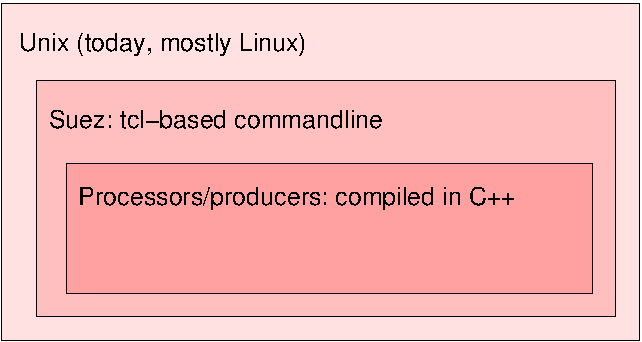
\includegraphics[width=0.7\linewidth]{environment}
\end{center}

\vfill
\begin{columns}
\column{0.85\linewidth}
This means a text editor will be your dearest friend

\vspace{0.25 cm}
though some processors have GUI interfaces
\begin{itemize}
\item Event Display
\item HistogramViewer
\end{itemize}

\column{0.2\linewidth}

\includegraphics[width=\linewidth]{gnu-head.pdf}
\end{columns}
\end{frame}

\begin{frame}
\frametitle{Suez data-access model}

Data which is valid for a given event is accessible through the Frame
(like a movie frame), and obsolete data is inaccessible.

\begin{center}
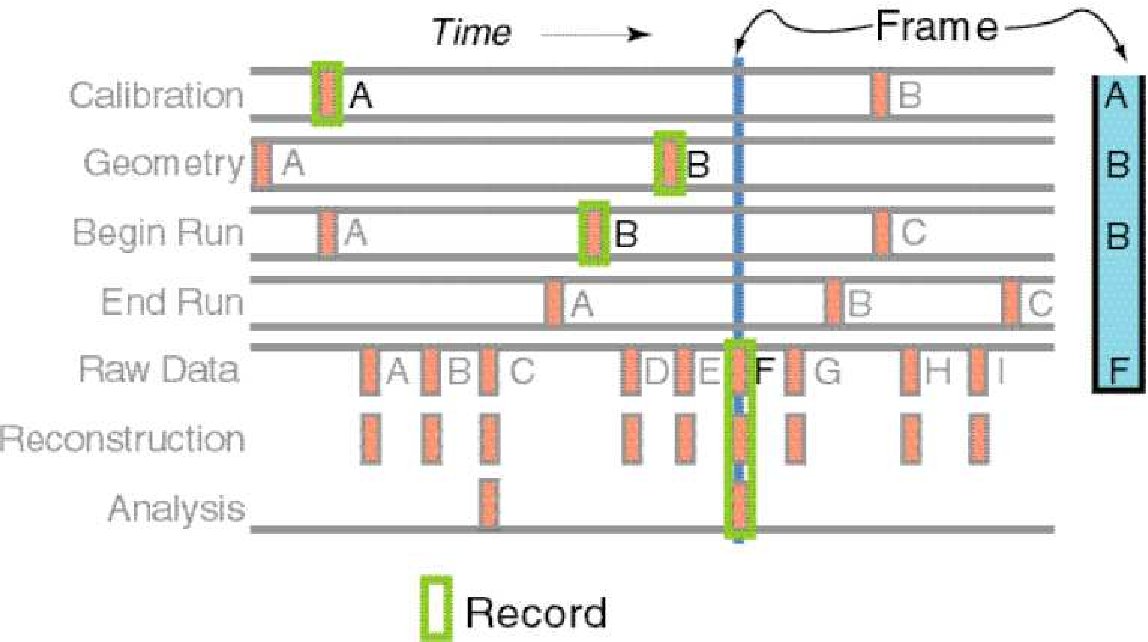
\includegraphics[width=\linewidth]{suezfigure}
\end{center}
\end{frame}

\begin{frame}
\frametitle{CMS, an LHC Detector Experiment}

Follows the same model (thanks to Chris Jones)
\begin{center}
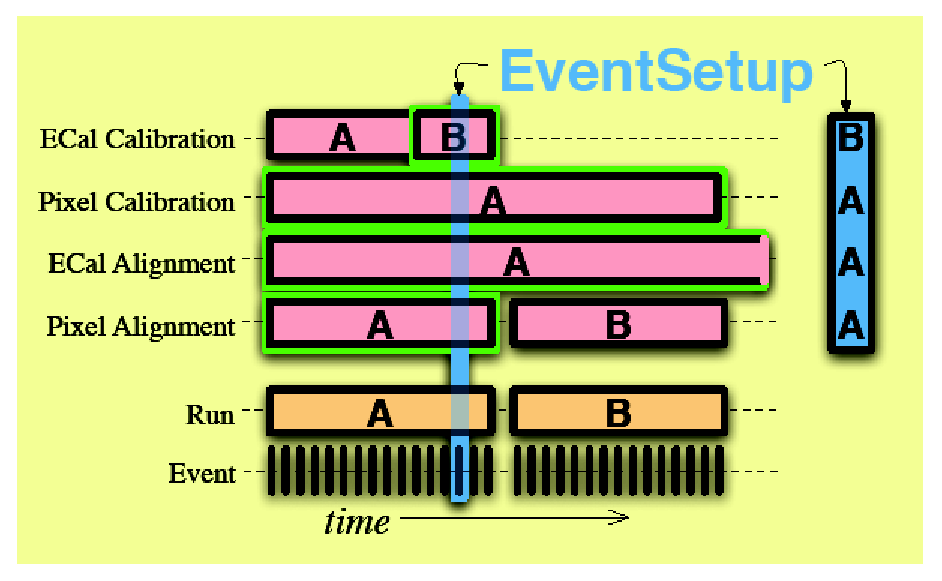
\includegraphics[width=\linewidth]{cmsfigure}
\end{center}
\end{frame}

\begin{frame}
\frametitle{Suez data processing model}

\begin{description}
\item[processors] are called in the event loop, extract data from the
  Frame, fill histograms, and filter events
\item[producers] are called when data is requested, extract what they
  need, and insert the desired results into the Frame
\item[modules] are the most general; we usually use them to read data
  from disk (EventStoreModule) and manage histogram output
  (RootHistogramModule)
\end{description}

\begin{center}
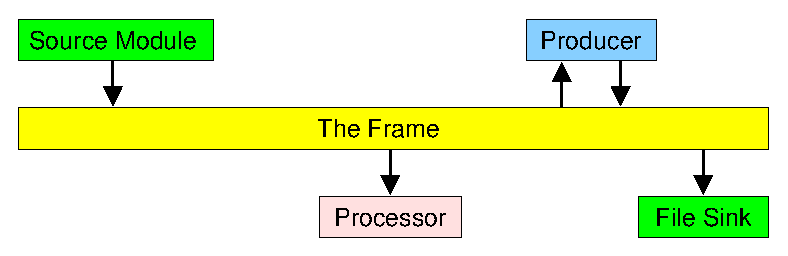
\includegraphics[width=0.7\linewidth]{procprod}
\end{center}
\end{frame}

\begin{frame}
\frametitle{A typical tcl (suez control file)}

\only<1>{\tt 

\mbox{\hspace{-0.175 cm}} \begin{minipage}{0.65\linewidth}
\begin{itemize}
\item module GoGetDataModule
\end{itemize}
\end{minipage}

\vspace{0.3 cm}
$\displaystyle \left.\mbox{\begin{minipage}{0.65\linewidth} \begin{itemize}
\item prod sel CalibrateDataProd
\item prod sel IdentifyTracksProd
\end{itemize} \end{minipage}} \right\} \mbox{\sf order does not matter}$

\vspace{0.2 cm}
$\displaystyle \left.\mbox{\begin{minipage}{0.78\linewidth} \begin{itemize}
\item proc sel FindGlueballsProc
\item proc sel MakePlotsOfGlueballsProc
\end{itemize} \end{minipage}} \right\} \mbox{\sf order matters}$

\vspace{0.2 cm}
$\displaystyle \left.\mbox{\begin{minipage}{0.78\linewidth} \begin{itemize}
\item go
\end{itemize} \end{minipage}} \right.$
}\only<2>{\tt 

\vspace{0.2 cm}
\mbox{\hspace{-0.175 cm}} \begin{minipage}{0.65\linewidth}
\begin{itemize}
\item module GoGetDataModule
\item prod sel CalibrateDataProd
\item prod sel IdentifyTracksProd
\item proc sel FindGlueballsProc
\item file out ToSkimFile
\item go
\end{itemize}
\end{minipage}
}

\sf
\vfill
\begin{center}
  \only<1>{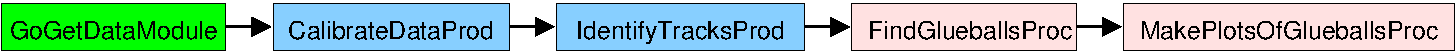
\includegraphics[width=\linewidth]{typicaltcl}}\only<2>{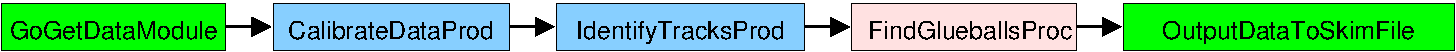
\includegraphics[width=\linewidth]{typicaltcl2}}
\end{center}

\vfill
\uncover<2>{Later, you can run {\tt MakePlotsOfGlueballsProc} on your
  skim file}

\end{frame}

\begin{frame}
\frametitle{Demonstration: The Event Display}

\begin{center}
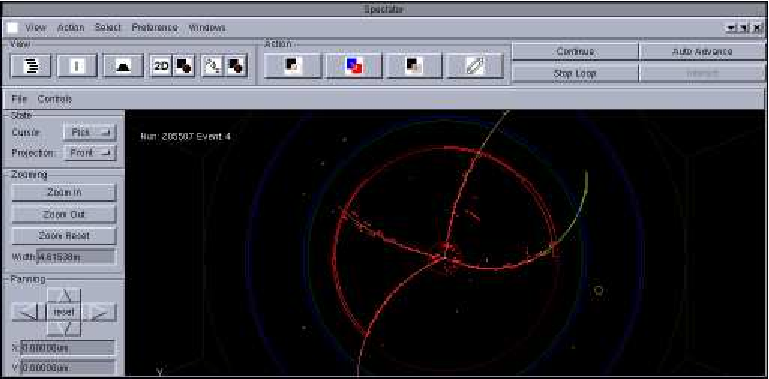
\includegraphics[width=0.8\linewidth]{eventdisplay}
\end{center}

The Event Display is a set of processors that draw CLEO data on the
screen, event by event.  It's useful for
\begin{itemize}
\item Data sanity check (e.g.\ during data-taking)
\item Identifying backgrounds
\item {\bf Introduction to CLEO/data analysis}
\end{itemize}

\end{frame}

\begin{frame}
\frametitle{Setup (review of yesterday)}

Connect to a Linux computer

\vfill
For {\bf \only<1>{bash/sh}\only<2>{tcsh/csh}} users (type ``{\tt echo \$SHELL}'' to identify),

{\tt \scriptsize
\begin{itemize}
\item \only<1>{. /nfs/cleo3/Offline/scripts/cleo3logins}\only<2>{source /nfs/cleo3/Offline/scripts/cleo3login}
\item \only<1>{. /nfs/cleo3/Offline/scripts/cleo3defs}\only<2>{source /nfs/cleo3/Offline/scripts/cleo3def}
\item \only<1>{c3rel 20060224\_FULL\_2}\only<2>{c3rel 20060224\_FULL\_2}
\item \only<1>{export USER\_SRC=\$HOME/my\_src}\only<2>{setenv USER\_SRC \$HOME/my\_src}
\item \only<1>{export USER\_BUILD=/cdat/tem/mccann/build/\$C3LIB}\only<2>{setenv USER\_BUILD /cdat/tem/mccann/build/\$C3LIB}
\item \only<1>{export USER\_SHLIB=\$USER\_BUILD/Linux/shlib}\only<2>{setenv USER\_SHLIB \$USER\_BUILD/Linux/shlib}
\item \only<1>{c3rel \$C3LIB}\only<2>{c3rel \$C3LIB} \hfill {\sf \it (yes, again!)}
\end{itemize}}

\vfill
Be sure to make the following directories (all shells):
{\tt \scriptsize
\begin{itemize}
\item mkdir -p \$HOME/my\_src
\item mkdir -p \$HOME/my\_tcl
\end{itemize}}
\end{frame}

\begin{frame}
\frametitle{Create a tcl file}

{\tt \scriptsize
\begin{itemize}
\item cd \$HOME/my\_tcl
\item favorite\_text\_editor hitsandeverything.tcl \&
\end{itemize}}

\vfill
Fill it with the following:

\vspace{0.5 cm}
\hspace{0.5 cm} \begin{minipage}{0.9\linewidth}
\tt \scriptsize
\textcolor{gray}{\# Get raw events so we can look at hits} \\
module sel EventStoreModule \\
eventstore in 20060601 daq all runs 205507 217380 \\
\mbox{ } \\
\textcolor{gray}{\# All the things you need to process raw data} \\
run\_file \$env(C3\_SCRIPTS)/getNewestConstants.tcl \\
run\_file \$env(C3\_SCRIPTS)/trackingDataFull.tcl \\
run\_file \$env(C3\_SCRIPTS)/CcP2.tcl \\
\mbox{ } \\
\textcolor{gray}{\# Run the event display} \\
run\_file \$env(C3\_SCRIPTS)/view\_command.tcl \\
view -display\_only ShowerAttributes DRHits ZDHits SeedTrack \\
\mbox{ } \hfill KinePionFit DBEventHeader StandAloneGeom

go
\end{minipage}
\end{frame}

\begin{frame}
\frametitle{Run Suez}

\begin{itemize}
\item {\tt suez -f hitsandeverything.tcl}
\end{itemize}

\begin{center}
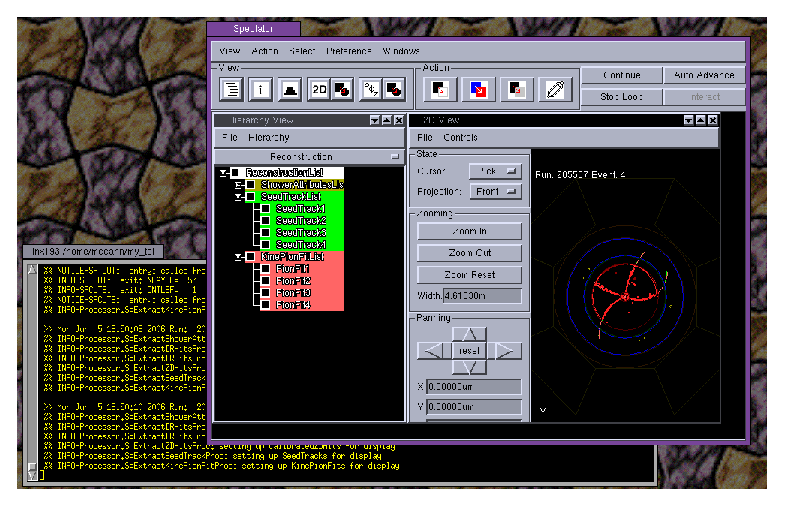
\includegraphics[width=\linewidth]{eventdisplay2}
\end{center}
\end{frame}

\begin{frame}
\frametitle{Things to do with the Event Display}
\begin{enumerate}\setlength{\itemsep}{0.4 cm}
\item Move windows within windows, zoom around, look at side view, select hits
\item Step through events (``Continue'' button); zip through them (``Auto Advance'' button)
\item SeedTracks (green) versus fitted tracks (KinePion, pink)
\item \label{showersarelabeled} Calorimeter shower representation: label with energy
\item \label{hitsarecircles} Make DR hits circles
\item \label{hitsarelines} Make ZD hits lines
\end{enumerate}
\end{frame}

\begin{frame}
\frametitle{The Drift Chamber} Wires strung between two endplates
report time of hit

which yields distance of closest approach of charged particle

\begin{center}
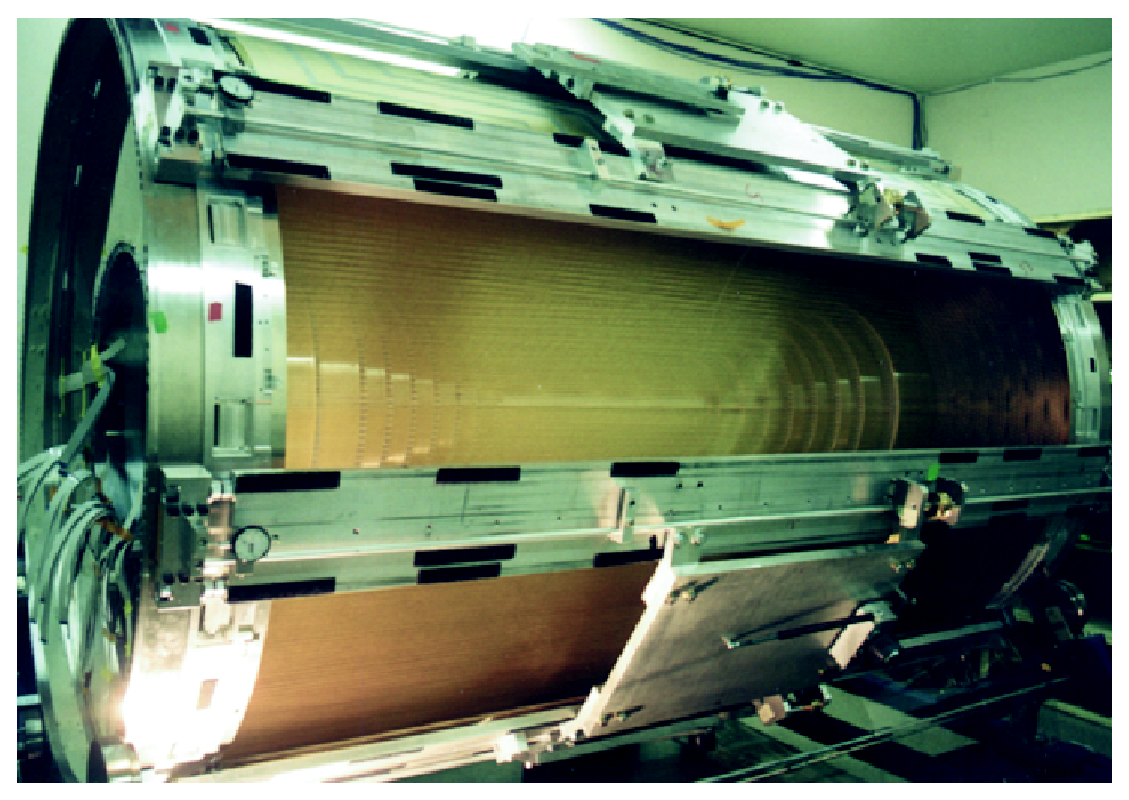
\includegraphics[width=0.9\linewidth]{cleo_dr}
\end{center}
\end{frame}

\begin{frame}
\frametitle{The Drift Chamber}
\begin{center}
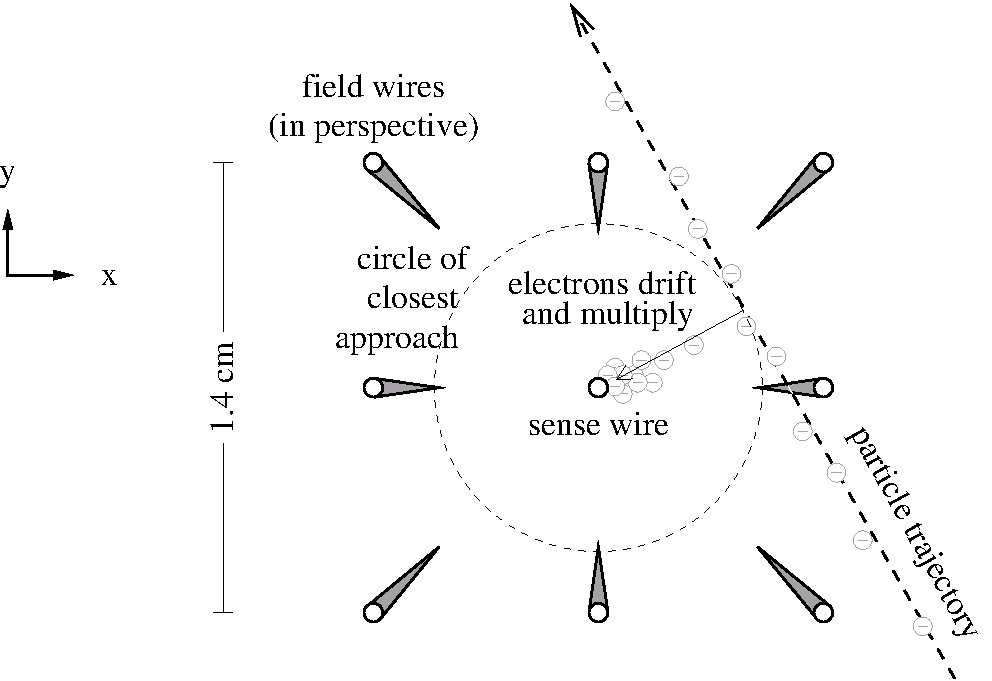
\includegraphics[width=\linewidth]{driftcell}
\end{center}
\end{frame}

\begin{frame}
\frametitle{The ZD} A small drift chamber with an extreme angle between the wire end positions (stereo angle)
\begin{center}
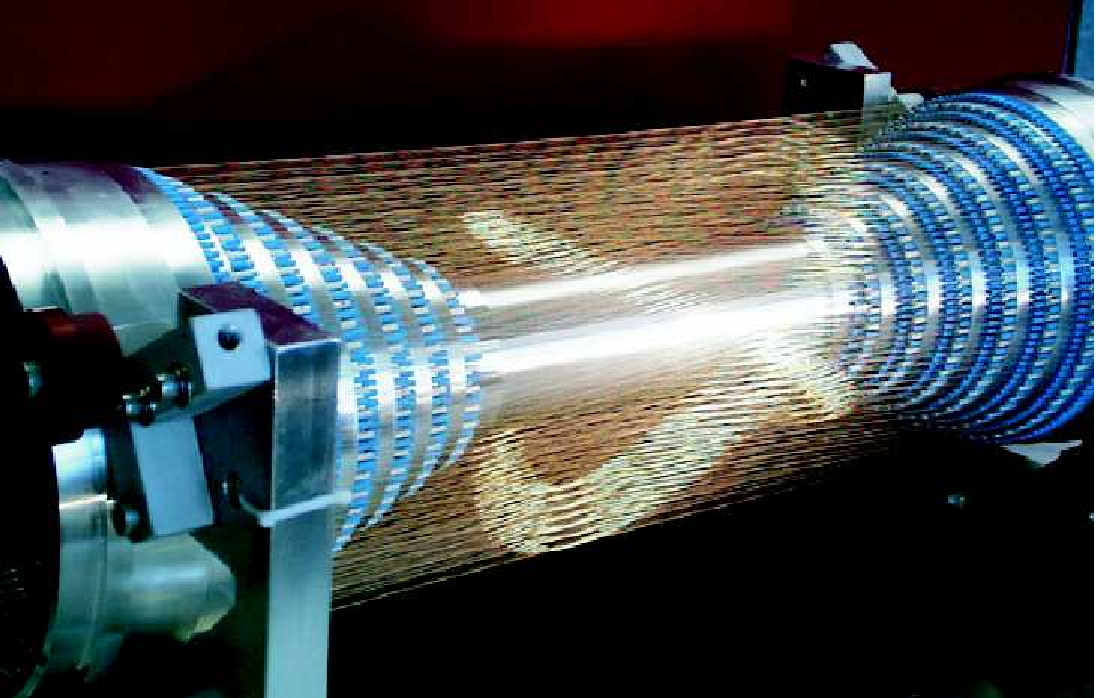
\includegraphics[width=0.9\linewidth]{cleo_zd}
\end{center}
\end{frame}

\begin{frame}
\frametitle{Stereo angle (detailed explaination)}
\begin{center}
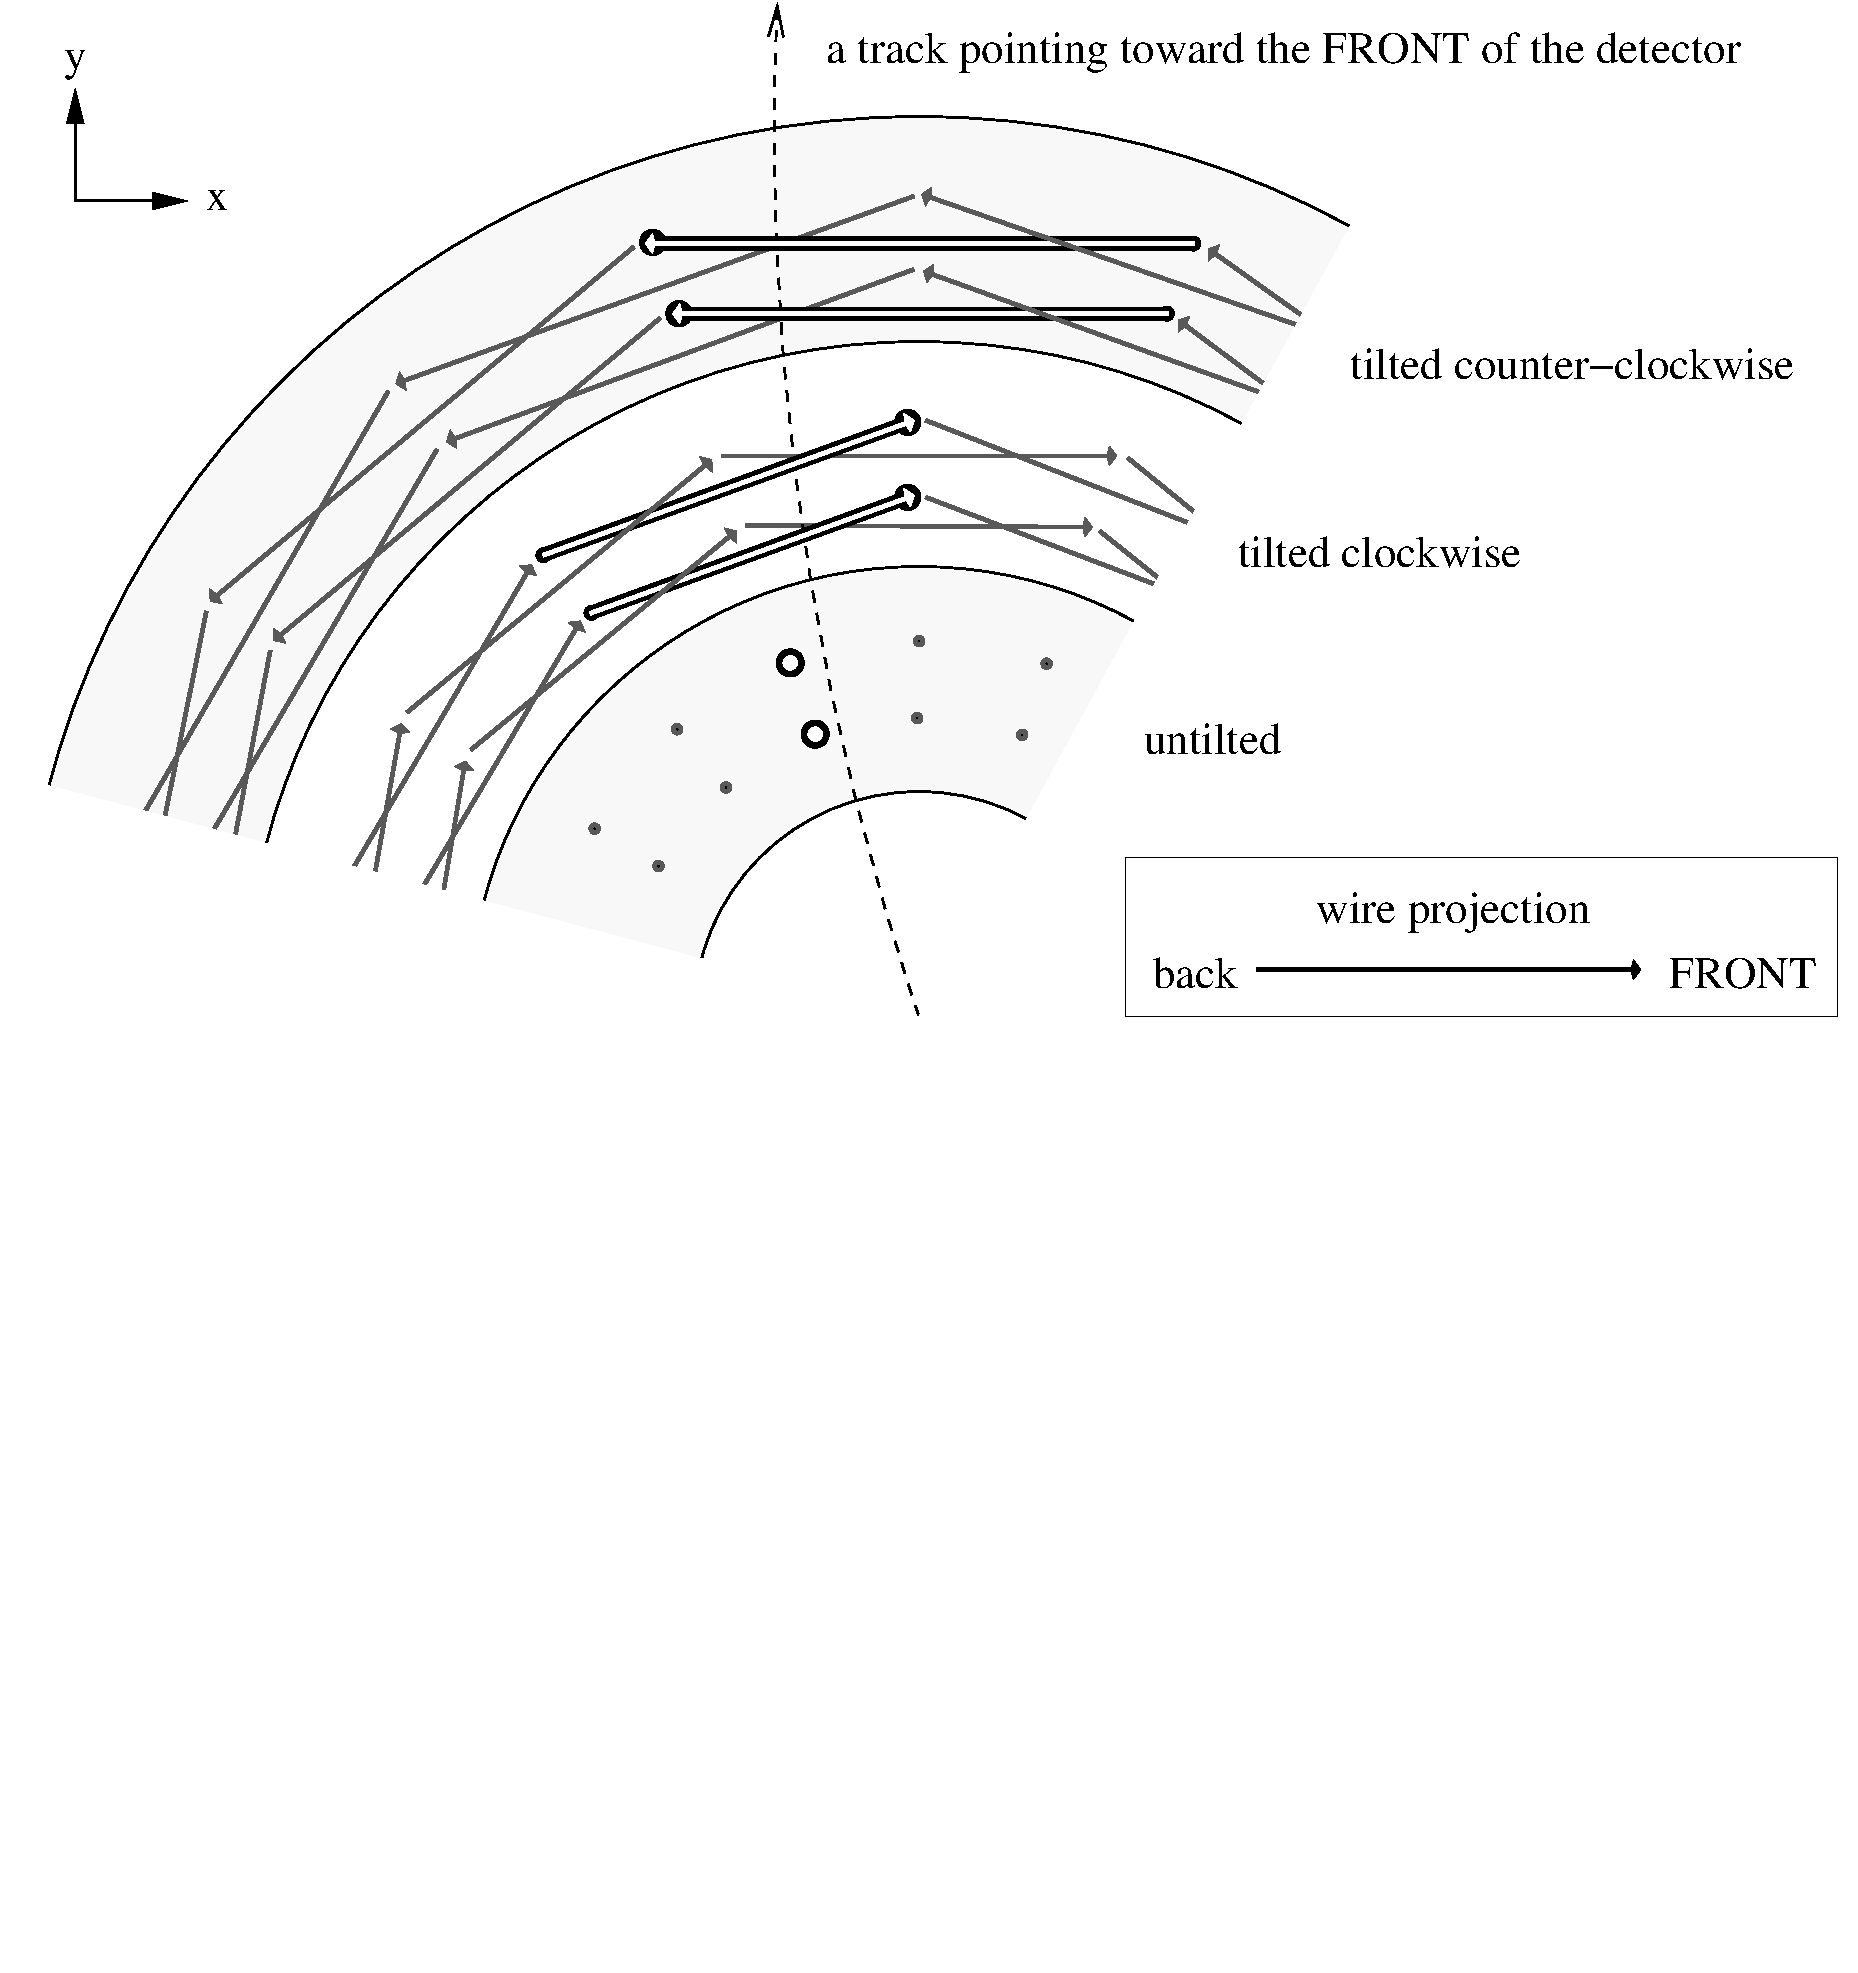
\includegraphics[width=0.9\linewidth, viewport=0 480 892 947]{stereotwist}
\end{center}

\vfill
\begin{minipage}{\linewidth}
\scriptsize Using tilted wires to obtain $z$ information in the outer
drift chamber/ZD.  Tilted wires extrude lines in the $x$-$y$
projection; position along a tilted wire indicates the $z$ of the
track helix near that wire.  The closest wires to the track (in three
dimensions) are highlighted.
\end{minipage}
\end{frame}

\begin{frame}
\frametitle{Cheat Sheet for \ref{showersarelabeled}, \ref{hitsarecircles}, and \ref{hitsarelines}}
View menu $\rightarrow$ Set 2D Representation\ldots

\begin{center}
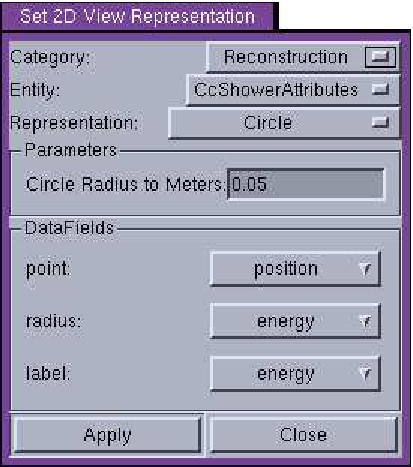
\includegraphics[width=0.3\linewidth]{showersarelabeled} \hfill 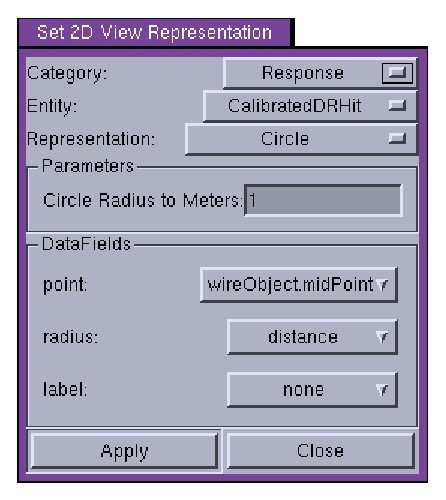
\includegraphics[width=0.3\linewidth]{hitsarecircles} \hfill 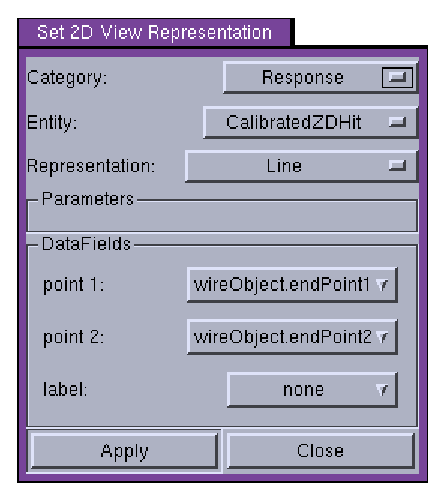
\includegraphics[width=0.3\linewidth]{hitsarelines}
\end{center}
\end{frame}

\begin{frame}
\frametitle{Pre-processed data: pass2}

{\tt \scriptsize
\begin{itemize}
\item cd \$HOME/my\_tcl
\item favorite\_text\_editor afterpass2.tcl \&
\end{itemize}}

\begin{minipage}{\linewidth}
\mbox{\hspace{1.2 cm}} \begin{minipage}{0.9\linewidth}
\tt \scriptsize
\textcolor{gray}{\# Get pass2'ed events (no hits, but much faster!)} \\
module sel EventStoreModule \\
eventstore in 20050316 physics all \\
\mbox{ } \\
\textcolor{gray}{\# Setup standard analysis and event display} \\
setup\_analysis \\
\mbox{ } \\
\textcolor{gray}{\# Run the event display} \\
run\_file \$env(C3\_SCRIPTS)/view\_command.tcl \\
view -display\_only Pass2 \\
\mbox{ } \\
go
\end{minipage}
\end{minipage}

\begin{itemize}
\item {\tt \scriptsize suez -f afterpass2.tcl}
\end{itemize}

\begin{enumerate}
\item Note the missing hits
\item See what happens when you press ``Auto Advance''
\end{enumerate}
\end{frame}

\begin{frame}
\frametitle{First Data Analysis}
Many events look like this:

\vfill
\begin{columns}[c]
\column{0.65\linewidth}
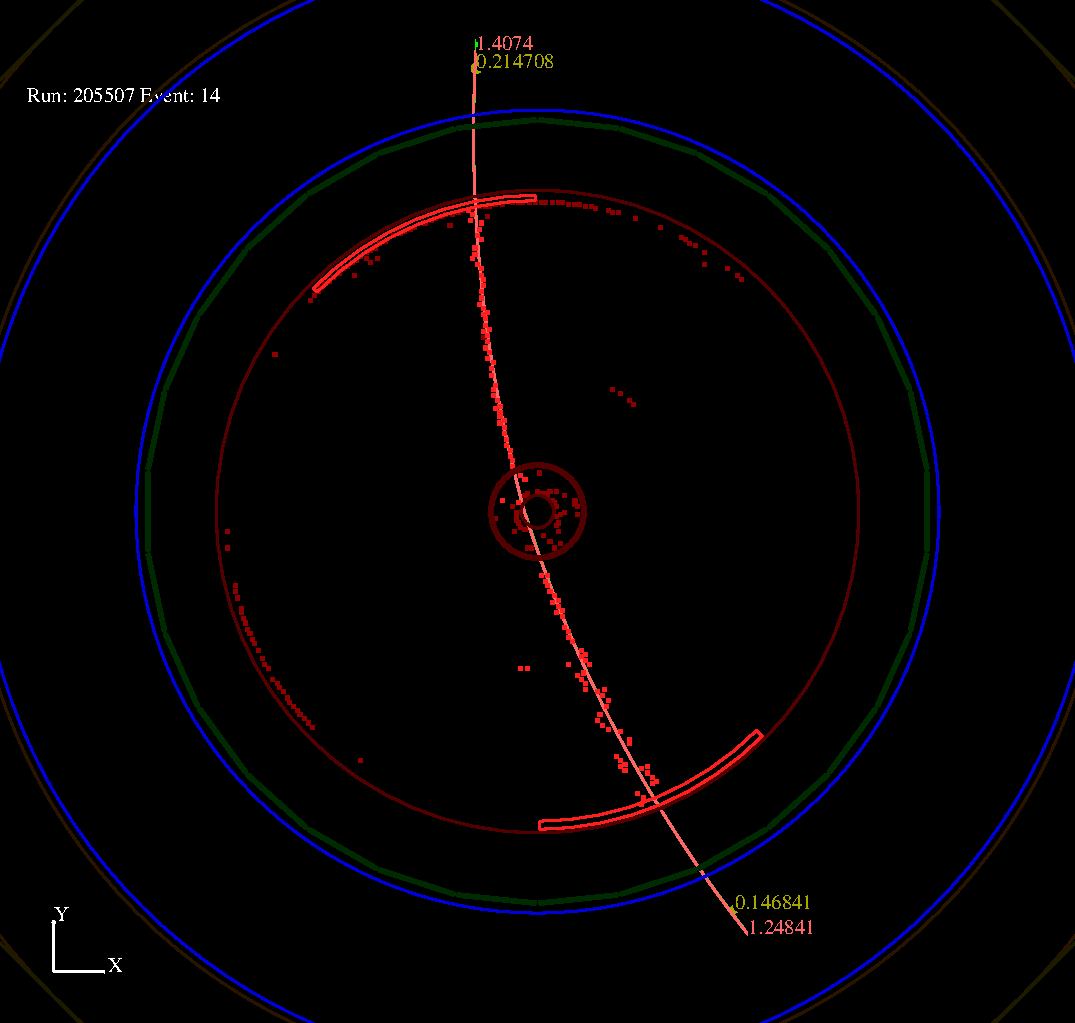
\includegraphics[width=\linewidth]{cosmicray}

\column{0.3\linewidth}
\begin{itemize}\setlength{\itemsep}{0.5 cm}
\item 2 tracks
\item minimal calorimeter energy \\ ($E/p$ $\lesssim$ 10\%)
\item misses the beamspot
\end{itemize}

\end{columns}
\end{frame}

\begin{frame}
\frametitle{Select Cosmic Rays}
We will make a processor that identifies cosmic rays

{\tt \scriptsize
\begin{itemize}
\item cd \$HOME/my\_src
\item mkproc -track -shower -histogram MySecondProcessor
\item favorite\_text\_editor MySecondProcessor/Class/MySecondProcessor.cc \&
\end{itemize}}

The processor is already filled with a lot of example code.  We'll
ignore that and add the following block at the beginning of the {\tt
MySecondProcessor::event} method (line 153).

Before editing, the code looks like this:
\vspace{0.5 cm}
\hspace{0.5 cm} \begin{minipage}{0.9\linewidth}
\tt \scriptsize
ActionBase::ActionResult \\
MySecondProcessor::event( Frame\& iFrame )          \textcolor{gray}{// anal3 equiv.} \\
\{ \\
\mbox{\hspace{0.25 cm}}report( DEBUG, kFacilityString ) $<<$ \rm \"\tt here in event()\rm \"\tt\ $<<$ endl;
\begin{center}
\textcolor{red}{$\rightarrow$ insert new code here $\leftarrow$}
\end{center}
\tt \mbox{\hspace{0.25 cm}}\textcolor{gray}{// Create a table of tracks and fill it.} \\
\mbox{\hspace{0.25 cm}}FATable$<$ NavTrack $>$ trackTable; \\
\mbox{\hspace{0.25 cm}}extract( iFrame.record( Stream::kEvent ) , trackTable );
\end{minipage}
\end{frame}

\begin{frame}
\frametitle{The New Code (page 1)}
\tt \scriptsize
\textcolor{darkgreen}{int} number\_of\_tracks = 0; \\
\textcolor{darkgreen}{double} closest\_to\_beamline = 1000.;  \textcolor{gray}{// meters} \\
\mbox{ } \\
\textcolor{darkgreen}{FATable$<$NavTrack$>$} tracks; \\
extract(iFrame.record(Stream::kEvent), tracks); \\
\mbox{ } \\
\textcolor{blue}{for} (\textcolor{darkgreen}{FATable$<$NavTrack$>$::const\_iterator} track = tracks.begin(); \\
\mbox{\hspace{1 cm}}track != tracks.end(); \\
\mbox{\hspace{1 cm}}++track) \{ \\
\mbox{ } \\
\mbox{\hspace{0.5 cm}}\textcolor{darkgreen}{double} distance\_from\_beamline = fabs(track-$>$pionHelix()-$>$d0()); \\
\mbox{\hspace{0.5 cm}}\textcolor{blue}{if} (distance\_from\_beamline $<$ closest\_to\_beamline) \{ \\
\mbox{\hspace{1 cm}}closest\_to\_beamline = distance\_from\_beamline; \\
\mbox{\hspace{0.5 cm}}\} \\
\mbox{ } \\
\mbox{\hspace{0.5 cm}}\textcolor{darkgreen}{double} track\_momentum = track-$>$pionFit()-$>$momentum().mag(); \\
\mbox{\hspace{0.5 cm}}\textcolor{blue}{if} (track\_momentum $>$ 1.) \{  \textcolor{gray}{// greater than 1 GeV/c} \\
\mbox{\hspace{1 cm}}number\_of\_tracks++; \\
\mbox{\hspace{0.5 cm}}\} \\
\} \\
\end{frame}

\begin{frame}
\frametitle{The New Code (page 2)}
\tt \scriptsize
\textcolor{darkgreen}{FATable$<$NavShower$>$} showers; \\
extract(iFrame.record(Stream::kEvent), showers); \\
\mbox{ } \\
\textcolor{darkgreen}{double} biggest\_shower\_energy = 0.;  \textcolor{gray}{// GeV} \\
\mbox{ } \\
\textcolor{blue}{if} (showers.size() $>$ 0) \\
\{ \\
\mbox{\hspace{0.5 cm}}\textcolor{gray}{// the showers table is sorted by energy} \\
\mbox{\hspace{0.5 cm}}biggest\_shower\_energy = showers.begin()-$>$attributes().energy(); \\
\} \\
\mbox{ } \\
\textcolor{gray}{// Now filter the events} \\
\textcolor{blue}{if} (number\_of\_tracks == 2  \&\& \hfill \begin{minipage}{5 cm}\textcolor{gray}{// two tracks above 1 GeV/c each}\end{minipage} \\
\mbox{\hspace{0.5 cm}} closest\_to\_beamline $>$ 0.05  \&\& \hfill \begin{minipage}{5 cm}\textcolor{gray}{// more than 5 cm from beamline}\end{minipage} \\
\mbox{\hspace{0.5 cm}} biggest\_shower\_energy $<$ 0.3) \hfill \begin{minipage}{5 cm}\textcolor{gray}{// less than 300 MeV}\end{minipage} \\
\{ \\
\mbox{\hspace{0.5 cm}}\textcolor{blue}{return} ActionBase::kPassed; \\
\} \\
else \\
\{ \\
\mbox{\hspace{0.5 cm}}\textcolor{blue}{return} ActionBase::kFailed; \\
\}
\end{frame}

\begin{frame}
\frametitle{Compile and Run}

{\tt \scriptsize
\begin{itemize}
\item c3make
\item cd \$HOME/my\_tcl
\item favorite\_text\_editor afterpass2.tcl \&
\end{itemize}}

\vfill In {\tt afterpass2.tcl}, add the processor after setting up the
view command but before calling it:

\vspace{0.25 cm}
\hspace{0.5 cm} \begin{minipage}{0.9\linewidth}
\tt \scriptsize
run\_file \$env(C3\_SCRIPTS)/view\_command.tcl \\
\textcolor{red}{proc sel MySecondProcessor} \\
view -display\_only Pass2
\end{minipage}

\vfill
Run suez
{\tt \scriptsize
\begin{itemize}
\item suez -f afterpass2.tcl
\end{itemize}}
and press the ``Auto Advance'' button in the Event Display.  See how you have biased the events!

\end{frame}

\begin{frame}
\frametitle{Histogram track $\phi$}

\begin{enumerate}\setlength{\itemsep}{0.4 cm}
\item \mbox{In {\tt \scriptsize \$HOME/my\_src/MySecondProcessor/MySecondProcessor/MySecondProcessor.h}, \hspace{-1 cm}} \\ add
{\tt \scriptsize HIHist1D* m\_histphi;} after {\tt \scriptsize HIHist1D* m\_histo1;}
\item \mbox{In {\tt \scriptsize \$HOME/my\_src/MySecondProcessor/Class/MySecondProcessor.cc},} add
{\tt \scriptsize m\_histphi = iHistoManager.histogram(\rm \"\tt phi\rm \"\tt , 100, 0., 2.*M\_PI);}
at the end of {\tt \scriptsize MySecondProcessor::hist\_book()\{ \}} (line 144)
\item Also add the following just before your \mbox{\tt \scriptsize \textcolor{blue}{return} ActionBase::kPassed;} (line 181)

\vspace{0.25 cm}
\hspace{0.5 cm} \begin{minipage}{0.9\linewidth}
\tt \scriptsize
\textcolor{blue}{for}
(\textcolor{darkgreen}{FATable$<$NavTrack$>$::const\_iterator} track = \\
\mbox{\hspace{1 cm}} tracks.begin(); track != tracks.end(); ++track) \\
\{ \\
\mbox{\hspace{0.5 cm}}m\_histphi-$>$fill(track-$>$pionHelix()-$>$phi0()); \\
\}
\end{minipage}

\item Recompile (described on previous page)
\end{enumerate}
\end{frame}

\begin{frame}
\frametitle{Histogram track $\phi$ (continued)}

\begin{enumerate}\addtocounter{enumi}{4}\setlength{\itemsep}{0.4 cm}
\item \mbox{At the beginning of {\tt \scriptsize \$HOME/my\_tcl/afterpass2.tcl}}, add

\vspace{0.25 cm}
\hspace{0.5 cm} \begin{minipage}{0.9\linewidth}
\tt \scriptsize
\textcolor{gray}{\# Load a histogram manager.} \\
module sel HbookHistogramModule \\
hbook file myhistograms.rzn \\
hbook init
\end{minipage}

\item Also add {\tt \scriptsize proc sel HistogramViewerProc} after \mbox{\tt \scriptsize proc sel MySecondProcessor}.

\item Run {\tt suez -f afterpass2.tcl} in your {\tt \$HOME/my\_tcl} directory.

\item Select Root $\rightarrow$ MySecondProcessor $\rightarrow$ phi
from the heirarchy on the left of the HistogramViewer window

\item Click ``Continue'' HistogramViewer and ``Auto Advance'' in the Event Display

\end{enumerate}
\end{frame}

\begin{frame}
\frametitle{Homework}

\begin{enumerate}\setlength{\itemsep}{0.3 cm}
\item Walk through the demonstrations on your own.
\item Study $e^+e^- \to \mu^+\mu^-$: plot the $\cos\theta$ distribution.

\vspace{0.2 cm}
Hints:\setlength{\itemsep}{0.4 cm}
\begin{itemize}\setlength{\itemsep}{0.1 cm}
\item Collision-borne muons deposit the same energy in calorimeter showers as cosmic ray muons.
\item But $e^+e^- \to \mu^+\mu^-$ events must come from the beam
\item Given a {\tt \scriptsize \textcolor{darkgreen}{FATable$<$NavTrack$>$::const\_iterator} track}, the momentum
vector components are obtained by {\tt \scriptsize track-$>$pionFit()-$>$momentum().x()}, {\tt \scriptsize .y()},
and {\tt \scriptsize .z()}.
\item $\theta$ is the polar angle between $\sqrt{x^2 + y^2}$ and $z$.
\item p.\ 137 Peskin \& Schroeder: $P(\cos\theta) \propto 1 + \cos^2\theta$
\end{itemize}

\end{enumerate}

\end{frame}

\begin{frame}
\frametitle{Shopping for data}
Very important webpages/directories

\begin{itemize}\setlength{\itemsep}{-0.25 cm}
\item Member functions:

\begin{itemize}
\item {\tt \scriptsize http://www.lns.cornell.edu/restricted/webtools/doxygen/ \\
\mbox{ } \hfill Offline/html/hierarchy.html}
\end{itemize}

\item Looking at the code:

\begin{itemize}
\item {\tt \scriptsize http://www.lns.cornell.edu/restricted/webtools/cleo3/}
\item {\tt \scriptsize ls \$C3\_CVSSRC/}
\item {\tt \scriptsize ls \$C3\_OTHER/}
\end{itemize}

\vspace{0.25 cm}
\item Producers to add to your {\tt .tcl}:

\begin{itemize}
\item {\tt \scriptsize http://www.lns.cornell.edu/$\sim$cleo3/current/data/ \\
\mbox{ } \hfill proxiesOfProducers.txt}
\end{itemize}

\item Event classification:

\begin{itemize}
\item {\tt \scriptsize http://www.lns.cornell.edu/restricted/CLEO/CLEO3/soft/hints/ \\
\mbox{ } \hfill CLEOIIIEventClassificationDescription.html}
\end{itemize}

\end{itemize}
\label{numpages}
\end{frame}

\end{document}
